\documentclass[10pt]{article}
\usepackage[a4paper,margin=0.72in]{geometry}
\usepackage{amsmath,amssymb}
\usepackage{booktabs}
\usepackage{graphicx}
\usepackage[hidelinks]{hyperref}
\usepackage{microtype}
\usepackage{enumitem}
\usepackage{array}
\usepackage{xcolor}
\usepackage{fancyvrb}

\graphicspath{{../figures/final/}{../figures/final/diagnostics/}}
\setlist{nosep,leftmargin=*}
\setlength{\parindent}{0pt}
\setlength{\parskip}{4pt}
\setlength{\textfloatsep}{7pt plus 2pt minus 2pt}
\setlength{\floatsep}{6pt plus 2pt minus 2pt}
\setlength{\intextsep}{6pt plus 2pt minus 2pt}
\newcolumntype{L}[1]{>{\raggedright\arraybackslash}p{#1}}

\title{\vspace{-1.2cm}Exact Encounter Analysis for Two Lazy Reflecting Walkers}
\author{}
\date{}

\begin{document}
\maketitle
\vspace{-1.3cm}

\section*{Conclusion}
For the current finite one-dimensional reflecting lattice with synchronous lazy
updates and co-location-only absorption, no robust \(F_2\) double peak was
found.  The unusual curves seen across Stage 1, Stage 2, and Stage 2b are best
explained as parity artifacts, same-target long tails, or weak target-shift
shoulders.  In particular, the representative boundary cases A--C are not
double peaks and are not classified as boundary-induced delayed channels; the
best retained target-shift case is only a weak shoulder, not a double peak.

The visible bumps or shoulders occur in specific regimes rather than as a
universal double-peak mechanism.  Short-distance, strongly asymmetric mobility
cases can show jagged raw peaks from odd/even parity; the negative control
\[
N=21,\qquad (a,b)=(6,2),\qquad q_1=0.02,\qquad q_2=0.90
\]
is the clearest example.  Slow near-boundary cases A--C show long tails or
shoulders, but the dominant encounter site is unchanged between early and late
windows: \(4\to4\), \(6\to6\), and \(3\to3\).  The best retained target-shift
case
\[
N=31,\qquad (a,b)=(2,4),\qquad q_1=0.70,\qquad q_2=0.20
\]
has a weak site shift \(4\to3\), but still no true \(F_2\) double peak.
Thus the jagged figure is normal for this synchronous discrete-time model: it
is a parity-comb artifact in raw \(f(t)\).  The decision curve is \(F_2\), which
pairs odd/even times before applying the repository's peak-valley rule.

\section*{Model and Exact Absorbing-Chain Formulation}
Sites are \(1,\ldots,N\).  Walker \(i\) has mobility \(q_i\in(0,1]\).  At an
interior site, the walker moves left/right with probabilities \(q_i/2\) and
stays with probability \(1-q_i\).  At the reflecting boundary, attempted
outside motion is converted into staying:
\[
P_i(1,1)=1-q_i/2,\quad P_i(1,2)=q_i/2,\qquad
P_i(N,N)=1-q_i/2,\quad P_i(N,N-1)=q_i/2.
\]
The synchronous independent update is
\[
P=P_1\otimes P_2.
\]
The transient set is the off-diagonal state space
\[
O=\{(x,y):x\neq y\},
\]
and the absorbing encounter set is
\[
D=\{(k,k):1\leq k\leq N\}.
\]
With \(Q=P[O,O]\) and \(R=P[O,D]\), the exact encounter-position distribution is
\[
f_k(t)=\alpha Q^{t-1}R_{\cdot,k},\qquad f(t)=\sum_k f_k(t).
\]
All reported curves and identities are exact sparse Markov-chain calculations,
not Monte Carlo estimates.

\section*{Spatial Configuration Views}
Figure~\ref{fig:spatial-configurations} shows the actual spatial configuration
for each selected case.  The left panel in each row is the physical reflecting
one-dimensional lattice: the two walker starts are marked, the reflecting walls
are drawn at sites \(1\) and \(N\), and the dominant early/late encounter sites
are shown directly on the lattice.  The right panel in each row is the ordered
Markov state space \((x,y)\).  Its diagonal is the absorbing co-location set
\(D=\{(k,k)\}\); the start is a single off-diagonal point.

\begin{figure}[!htbp]
  \centering
  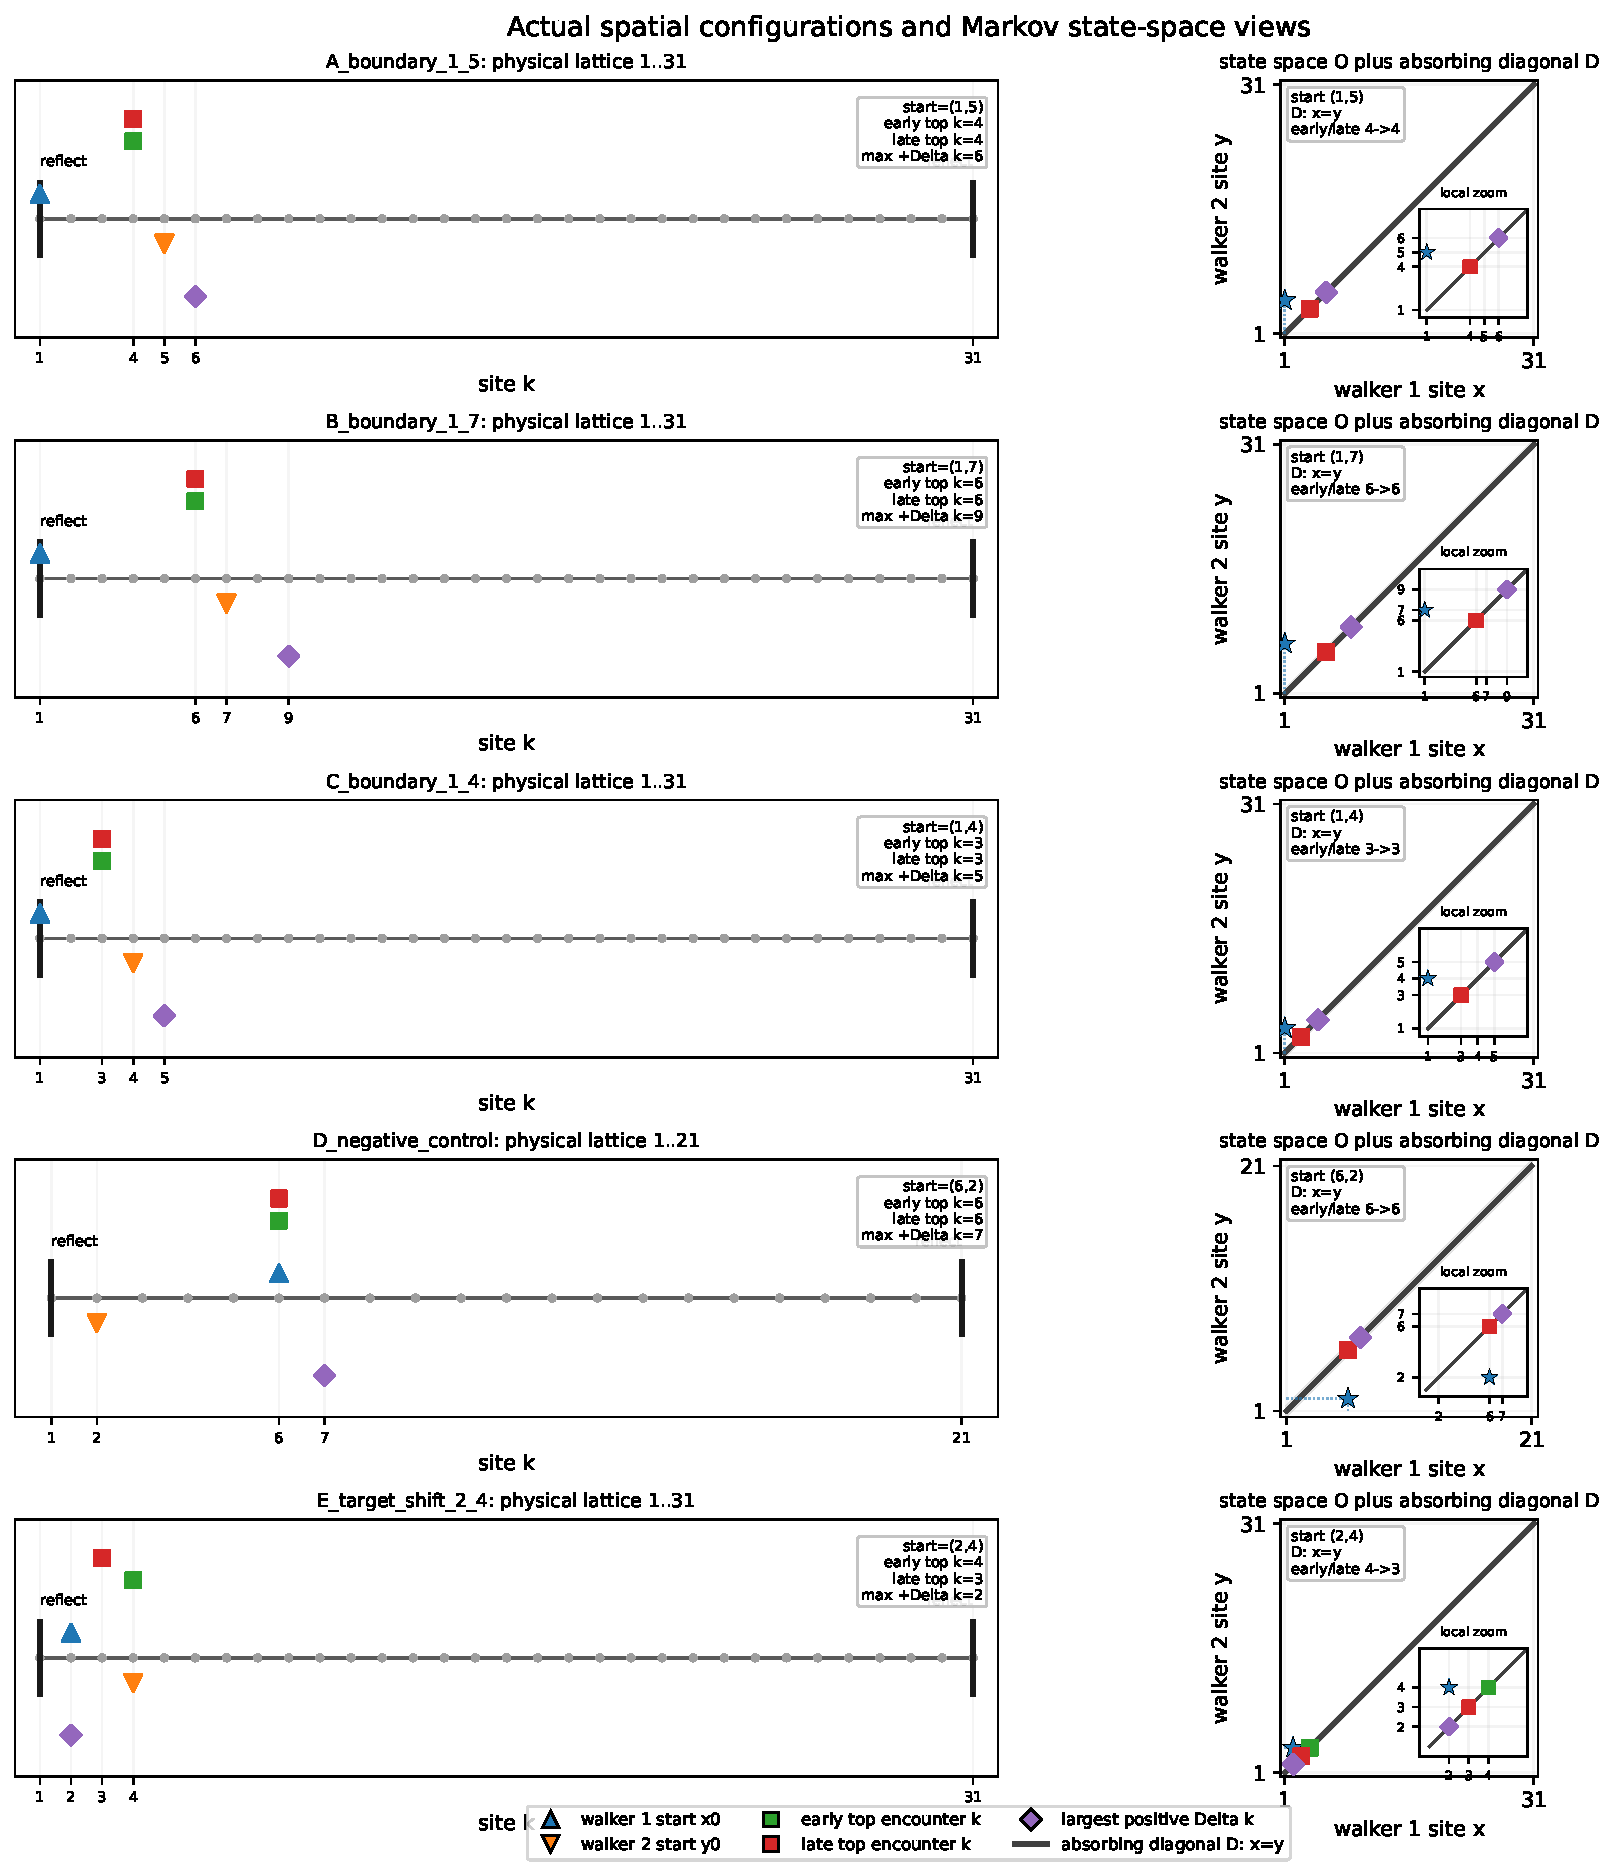
\includegraphics[width=0.96\linewidth]{spatial_configurations.pdf}
  \caption{Actual spatial configurations.  Left: physical 1D lattice.  Right:
  ordered state space \((x,y)\), where the diagonal is the absorbing encounter
  set.  Marker meanings are shown in the legend: blue up-triangle is walker 1
  start \(x_0\), orange down-triangle is walker 2 start \(y_0\), green square is
  early top encounter site, red square is late top encounter site, and purple
  diamond is the site with largest positive
  \(\Delta_k=C_{\rm late}-C_{\rm early}\).  Each right panel also includes a
  local zoom near the start and dominant encounter sites.}
  \label{fig:spatial-configurations}
\end{figure}

\section*{Operational Double-Peak Rule and Figure Reading}
A raw second bump is not enough.  The final rule first forms the parity-pair
curve
\[
F_2(n)=f(2n-1)+f(2n),
\]
which removes odd/even synchronous-update oscillations.  A case is called a
robust \(F_2\) double peak only if all of the following hold:
\begin{enumerate}
  \item \(F_2\) has a main local maximum and a later true local maximum.
  \item The later maximum is more than two \(F_2\) bins after the main peak.
  \item The later peak height is at least \(5\%\) of the main peak height.
  \item The valley between the two peaks is at most \(80\%\) of the smaller
  peak height.
\end{enumerate}
If these conditions fail, the feature is reported as a shoulder, long tail,
target-shift shoulder, or artifact.  This is why cases A--C and the best
target-shift case are not called double peaks.

This is aligned with the repository's existing visual double-peak convention,
\(\rho=h_v/\min(h_1,h_2)\leq 0.8\).  The encounter-specific part is only the
preprocessing step: synchronous co-location curves can alternate strongly
between odd and even time steps, so the final double-peak claim applies the
same peak-valley rule to \(F_2\), not directly to raw \(f(t)\).

In the diagnostic figures, dashed green/red vertical lines mark the main and
late diagnostic times.  The \(C_k\) panel compares normalized encounter-site
mass in the early and late windows.  The heatmap is \(\log_{10} f_k(t)\), so it
is meant to show which encounter sites carry mass at each time rather than to
show a probability density on a linear colour scale.  Light gray bands and
inset axes mark local zoom windows for the jagged, shoulder, or \(F_2\)-decision
regions that are hard to inspect on the full time axis.

\section*{Formula and Green-Function Validation}
The fundamental-matrix identities are
\[
\mathbb{E}[T]=\alpha (I-Q)^{-1}{\bf 1},\qquad
p_k=\alpha (I-Q)^{-1}R_{\cdot,k},
\]
and
\[
\tau_k
=\frac{\alpha (I-Q)^{-1}(I-Q)^{-1}R_{\cdot,k}}{p_k}.
\]
The validation table shows numerical closure of mass, mean, encounter-position
probabilities, and the \(p_k\tau_k\) decomposition.

\begin{table}[!htbp]
\centering
\footnotesize
\caption{Formula validation.  Errors are at floating-point scale.}
\begin{tabular}{L{2.8cm}rrrrr}
\toprule
case & \(N\) & \(\sum_t f(t)\) & tail mass & mean error & \(p\tau\) mean error\\
\midrule
L5 edge q04 q09 & 5 & 1.000000 & \(9.42{\times}10^{-13}\) & \(2.50{\times}10^{-10}\) & \(8.88{\times}10^{-15}\)\\
L6 inner q07 q03 & 6 & 1.000000 & \(9.78{\times}10^{-13}\) & \(4.58{\times}10^{-10}\) & \(2.13{\times}10^{-14}\)\\
L7 asym q02 q08 & 7 & 1.000000 & \(9.63{\times}10^{-13}\) & \(6.25{\times}10^{-10}\) & \(4.97{\times}10^{-14}\)\\
\bottomrule
\end{tabular}
\end{table}

For \(N=5\), start \((1,5)\), \(q_1=0.4\), \(q_2=0.9\), the absorbing-chain
probability-generating function agrees with the determinant Green-function
formula.  The maximum absolute error over \(z=0.2,0.5,0.8,0.95\) is
\(3.52\times 10^{-16}\).

\begin{table}[!htbp]
\centering
\footnotesize
\caption{Green-function determinant validation.}
\begin{tabular}{rrrr}
\toprule
\(z\) & absorbing PGF & determinant PGF & absolute error\\
\midrule
0.20 & 0.000789 & 0.000789 & \(3.52{\times}10^{-16}\)\\
0.50 & 0.015682 & 0.015682 & \(5.20{\times}10^{-17}\)\\
0.80 & 0.150581 & 0.150581 & \(2.78{\times}10^{-16}\)\\
0.95 & 0.562263 & 0.562263 & \(1.11{\times}10^{-16}\)\\
\bottomrule
\end{tabular}
\end{table}

\section*{Mean Encounter Time Versus Mobility Ratio}
The mean-ratio pilot shows that an interior maximum of the exact mean encounter
time is not universal.  Two starts have an interior maximum over the scanned
range; the boundary-to-boundary fixed-sum case has an interior minimum and an
endpoint maximum.

\begin{figure}[!htbp]
  \centering
  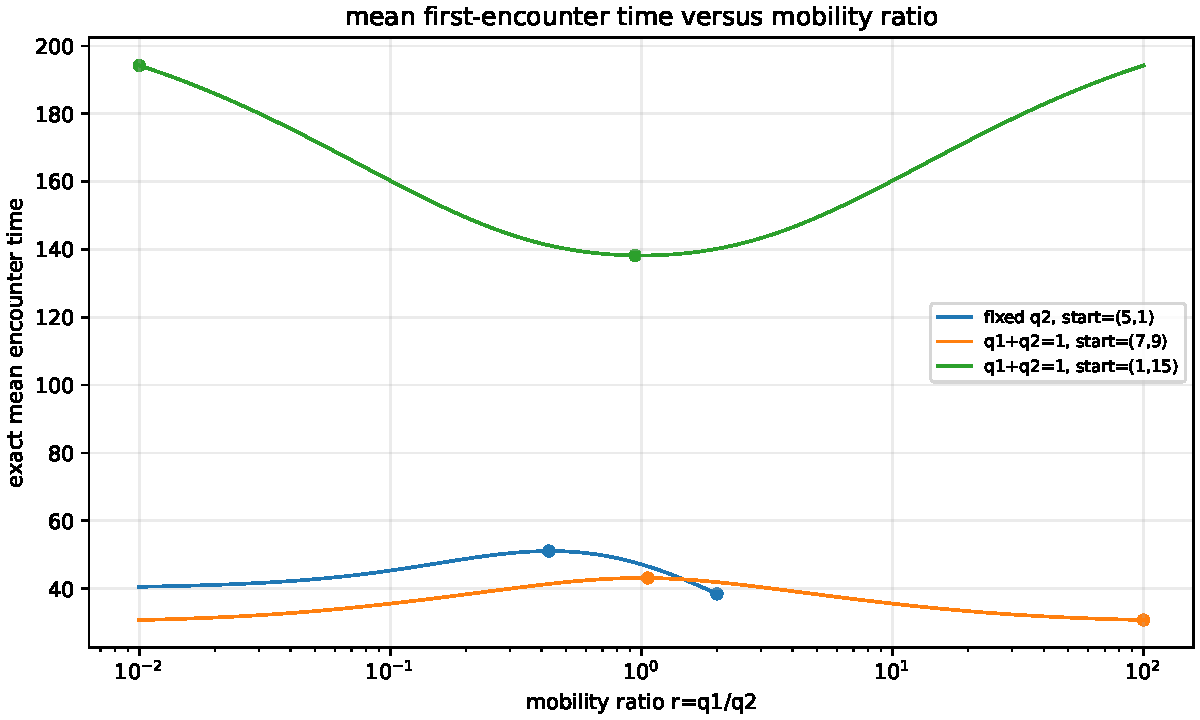
\includegraphics[width=0.82\linewidth]{mean_vs_ratio.pdf}
  \caption{Exact mean encounter time as a function of the mobility ratio
  \(r=q_1/q_2\) for the three pilot scans.}
\end{figure}

\begin{table}[!htbp]
\centering
\footnotesize
\caption{Mean-ratio extrema.}
\begin{tabular}{L{4.0cm}L{3.0cm}rrr}
\toprule
scan & extremum & \(r\) & \(q_1\) & mean\\
\midrule
fixed \(q_2\), start \((5,1)\) & global/local max & 0.427671 & 0.213836 & 51.0852\\
fixed \(q_2\), start \((5,1)\) & global min & 2.000000 & 1.000000 & 38.4629\\
fixed sum, start \((7,9)\) & global/local max & 1.060026 & 0.514569 & 43.1421\\
fixed sum, start \((7,9)\) & global min & 100.000000 & 0.990099 & 30.7548\\
fixed sum, start \((1,15)\) & global max & 0.010000 & 0.009901 & 194.223\\
fixed sum, start \((1,15)\) & global/local min & 0.943373 & 0.485431 & 138.226\\
\bottomrule
\end{tabular}
\end{table}

\section*{Why the Stage-1 Double Peaks Were Artifacts}
Stage 1 ranked raw curve shapes.  This promoted short-distance parity combs:
raw \(f(t)\) has repeated alternating local maxima, but the parity-pair curve
\[
F_2(n)=f(2n-1)+f(2n)
\]
collapses the pattern to a single meaningful peak.  These rows are therefore
rejected as parity or ballistic-short-distance artifacts.

\begin{figure}[!htbp]
  \centering
  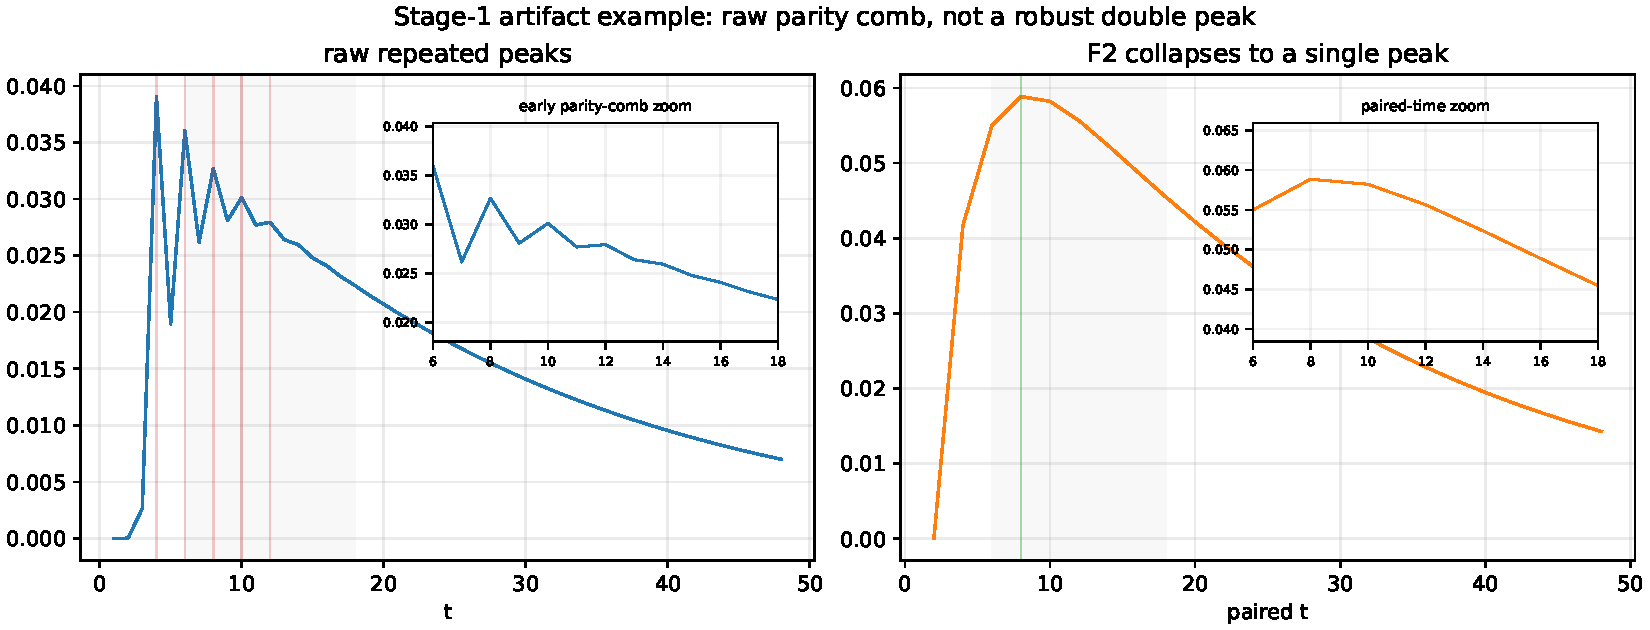
\includegraphics[width=0.82\linewidth]{stage1_artifact_raw_vs_f2.pdf}
  \caption{Stage-1 artifact example.  Multiple raw peaks disappear after
  pairing adjacent odd/even times into \(F_2\).  Insets enlarge the early
  parity-comb region and the paired-time decision region.}
\end{figure}

\section*{Stage-2 and Stage-2b: No Robust \(F_2\) Double Peaks}
Stage 2 introduced smoothing persistence, parity-pair filtering, and negative
controls.  Stage 2b added mechanism-focused checks: boundary-null controls,
target-shift reranking, encounter-site windows, grouped \(f_G(t)\) curves, and
leading eigenmodes of \(Q\).  In the Stage-2b case table plus the top-30
target-shift table, the number of robust \(F_2\) double peaks is zero.

\begin{table}[!htbp]
\centering
\footnotesize
\caption{Final mechanism classification for the representative cases.}
\begin{tabular}{L{3.1cm}L{2.7cm}rrrrr}
\toprule
case & class & \(N\) & start & \(q_1\) & \(q_2\) & top \(k\) early/late\\
\midrule
A boundary 1--5 & same-target tail & 31 & \((1,5)\) & 0.05 & 0.02 & \(4\to4\)\\
B boundary 1--7 & same-target tail & 31 & \((1,7)\) & 0.10 & 0.02 & \(6\to6\)\\
C boundary 1--4 & same-target tail & 31 & \((1,4)\) & 0.05 & 0.02 & \(3\to3\)\\
D negative control & parity artifact & 21 & \((6,2)\) & 0.02 & 0.90 & \(6\to6\)\\
best target shift & weak target-shift shoulder & 31 & \((2,4)\) & 0.70 & 0.20 & \(4\to3\)\\
\bottomrule
\end{tabular}
\end{table}

\section*{Same-Target Long-Tail Cases A--C}
Cases A--C are shoulders or long tails, not double peaks.  Their early and late
encounter-site distributions have the same dominant \(k\), and the translated
interior controls do not show a large boundary-specific amplification.  They
are therefore not called boundary-induced delayed channels.

\begin{figure}[!htbp]
  \centering
  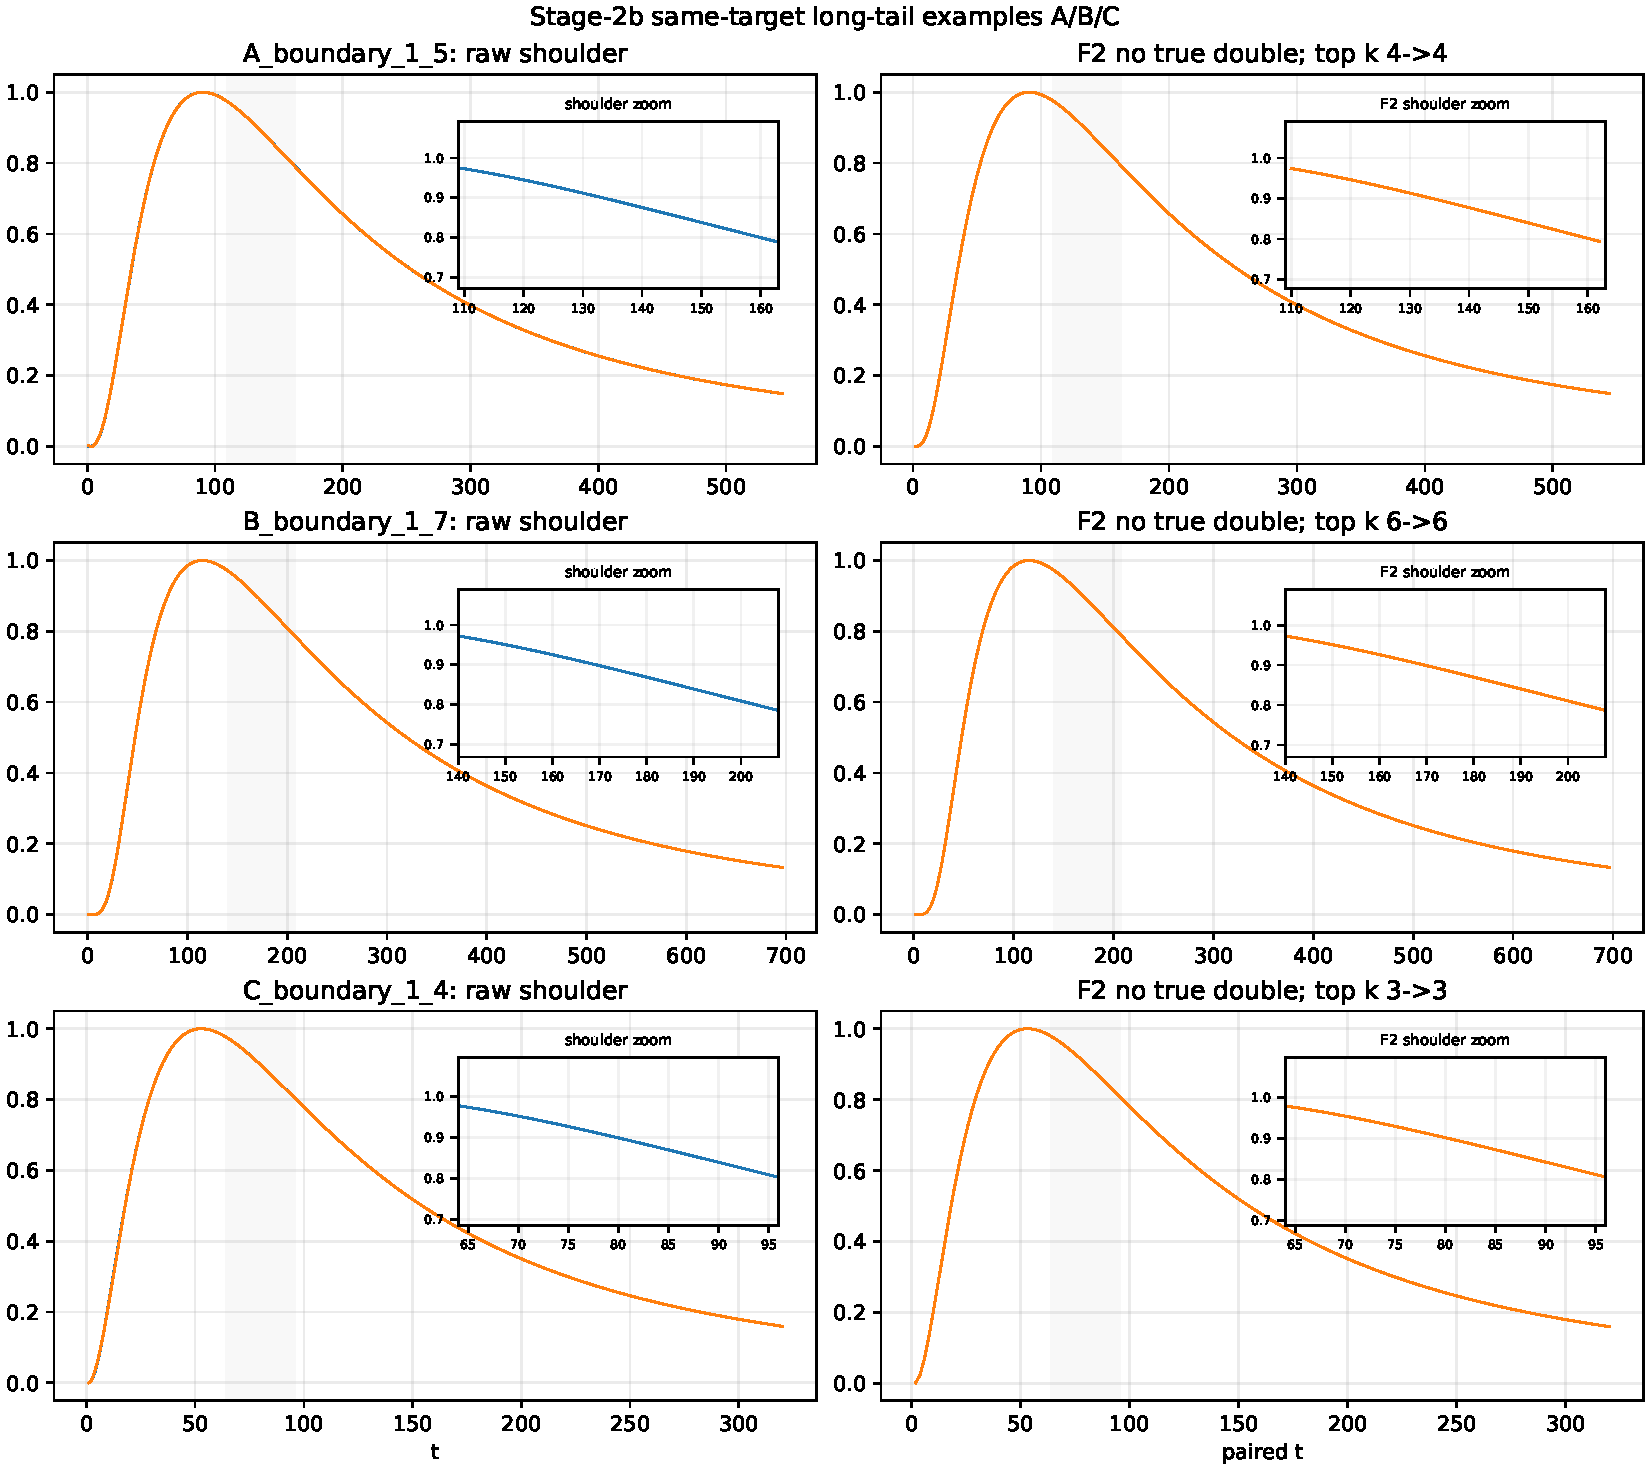
\includegraphics[width=0.9\linewidth]{same_target_tail_ABC.pdf}
  \caption{Same-target long-tail examples A--C.  The raw curves have late
  shoulders, but \(F_2\) has no true second local maximum with a visible valley.
  Insets zoom the shoulder windows.}
\end{figure}

\begin{figure}[!htbp]
  \centering
  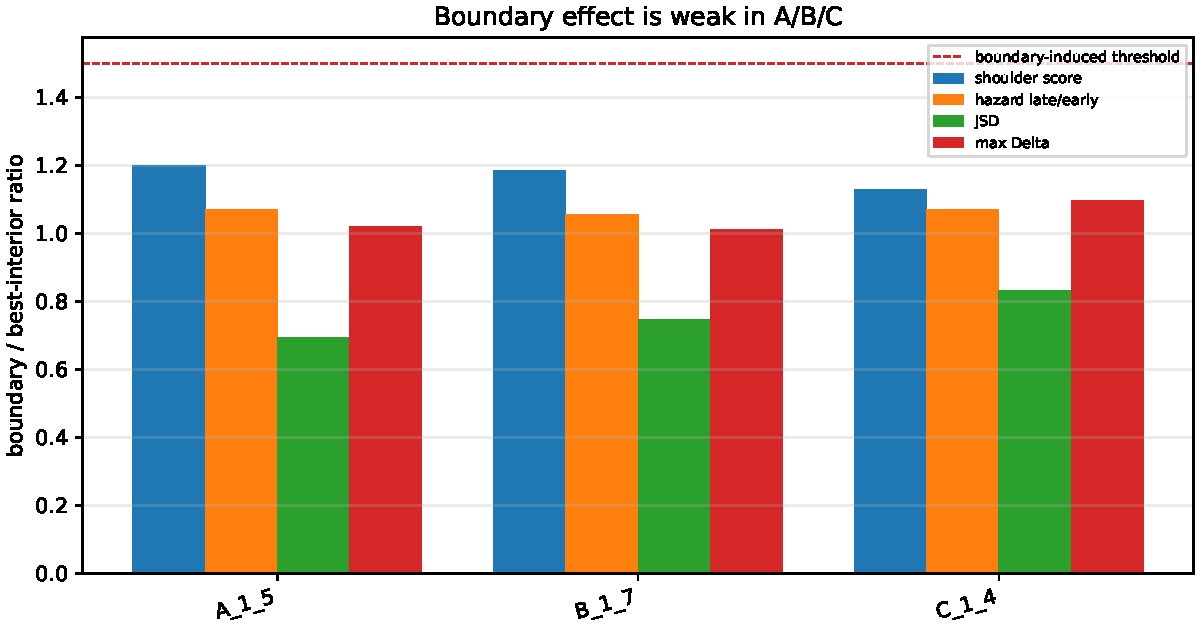
\includegraphics[width=0.78\linewidth]{boundary_vs_interior_summary.pdf}
  \caption{Boundary-null comparison.  The boundary cases do not dominate their
  translated interior controls strongly enough to support a boundary-induced
  mechanism.}
\end{figure}

\section*{Weak Target-Shift Shoulder}
The clearest retained target-shift case is
\[
N=31,\qquad (a,b)=(2,4),\qquad q_1=0.7,\qquad q_2=0.2.
\]
Its early/late encounter-site distributions shift from top site \(k=4\) to
\(k=3\), with \(JSD=0.0537\), maximum positive \(\Delta_k\) at \(k=2\), and
target-shift score \(1.43\times10^{-3}\).  This is a weak target-shift
shoulder, not a double peak: \(F_2\) still lacks two true local maxima separated
by a visible valley.

\begin{figure}[!htbp]
  \centering
  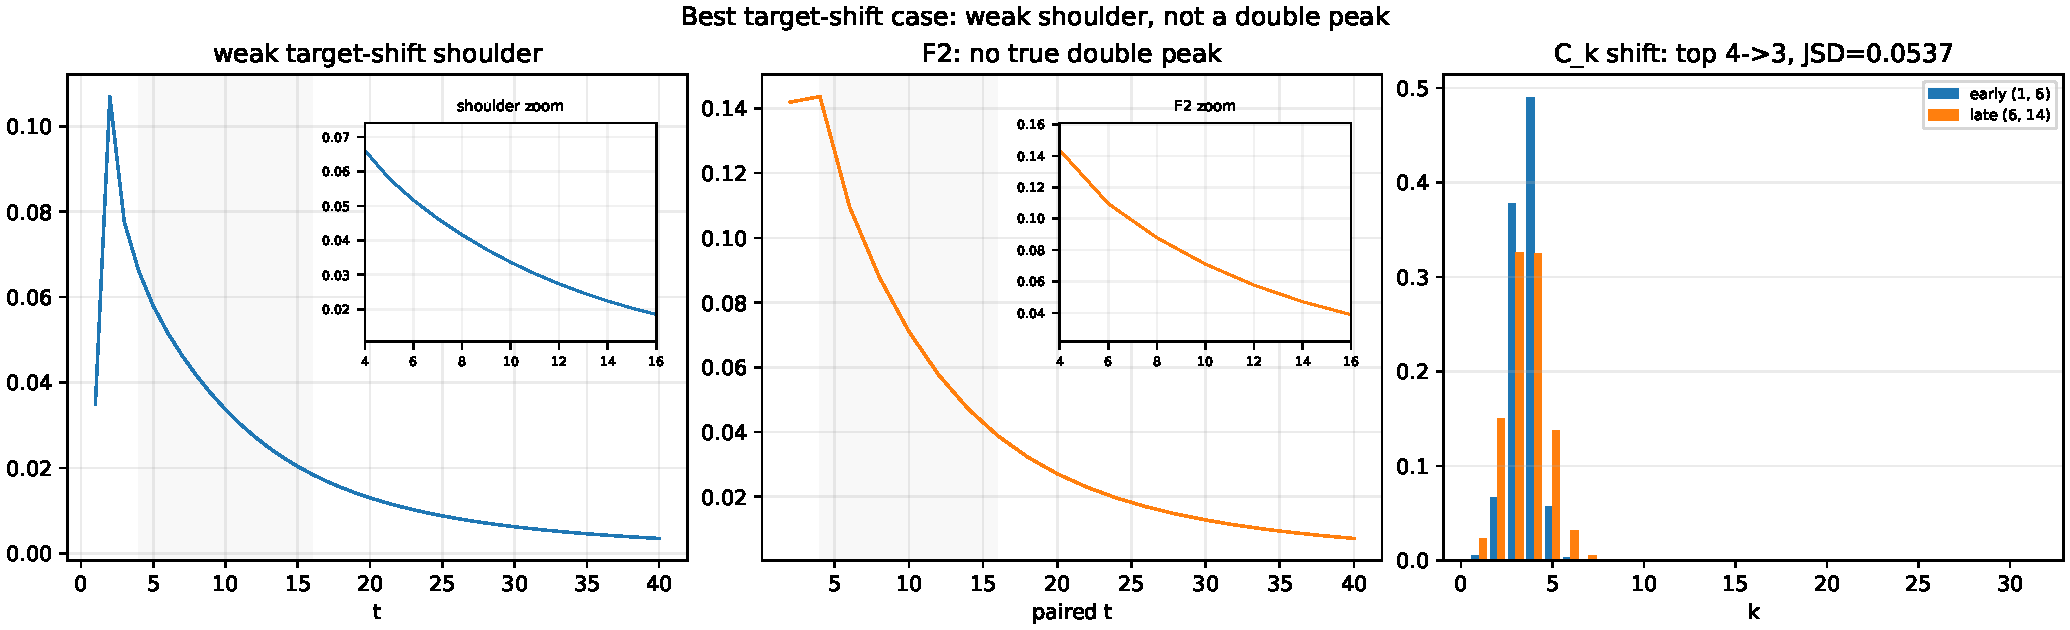
\includegraphics[width=0.9\linewidth]{best_target_shift.pdf}
  \caption{Best target-shift example.  The \(C_k\) distribution shifts, but the
  total curve does not become a robust \(F_2\) double peak.  Insets zoom the
  weak shoulder and \(F_2\)-decision windows.}
\end{figure}

\section*{Spectral Interpretation}
The leading eigenvalues of \(Q\) are close to one, and the late curves are
consistent with slow-mode relaxation rather than a separate second-peak
mechanism.  For case A, the leading mode has
\(\lambda=0.99982753\) and top \(R\)-channel \(k=16\), while the early and late
dominant encounter site remains \(k=4\).  The target-shift example shows a
modest \(C_k\) redistribution, but not a distinct slow channel that creates a
true second peak.

\begin{figure}[!htbp]
  \centering
  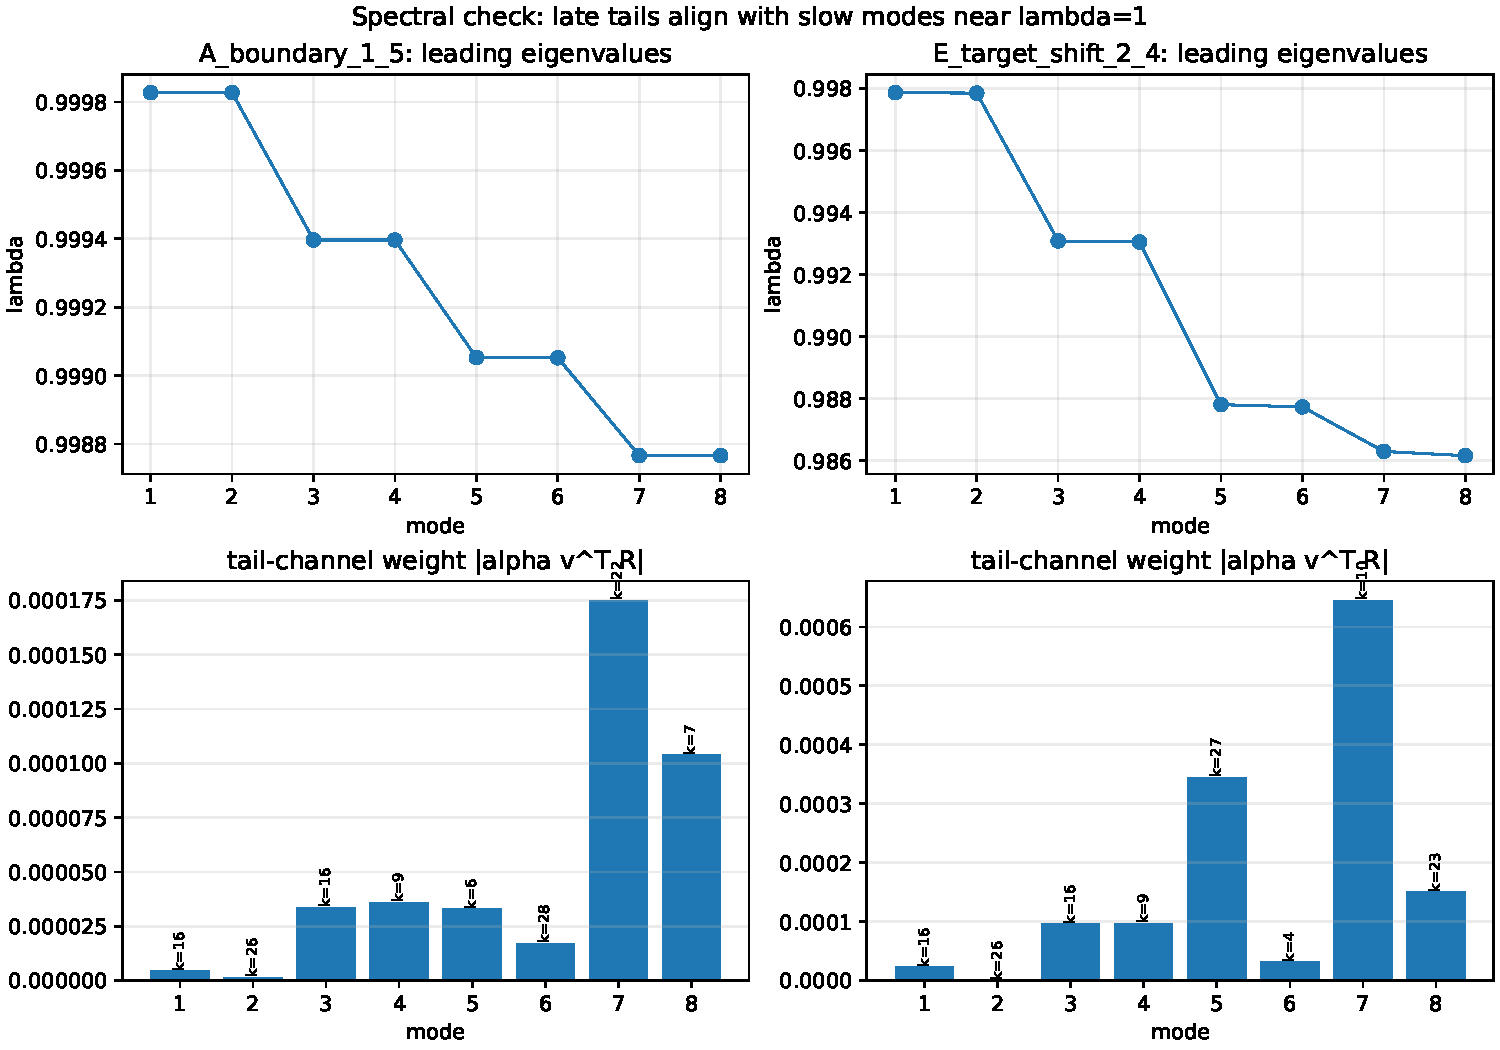
\includegraphics[width=0.86\linewidth]{spectral_A_and_target_shift.pdf}
  \caption{Leading eigenmodes for case A and the best target-shift shoulder.}
\end{figure}

\section*{Diagnostic Appendix}
The appendix figures show, for each selected case, raw \(f(t)\), smoothed
\(f(t)\), \(F_2\), \(\log f(t)\), hazard \(h(t)=f(t)/S(t-1)\), log-derivative
of \(F_2\), \(k\)-time heatmap, and early/late \(C_k\).

\begin{figure}[p]
  \centering
  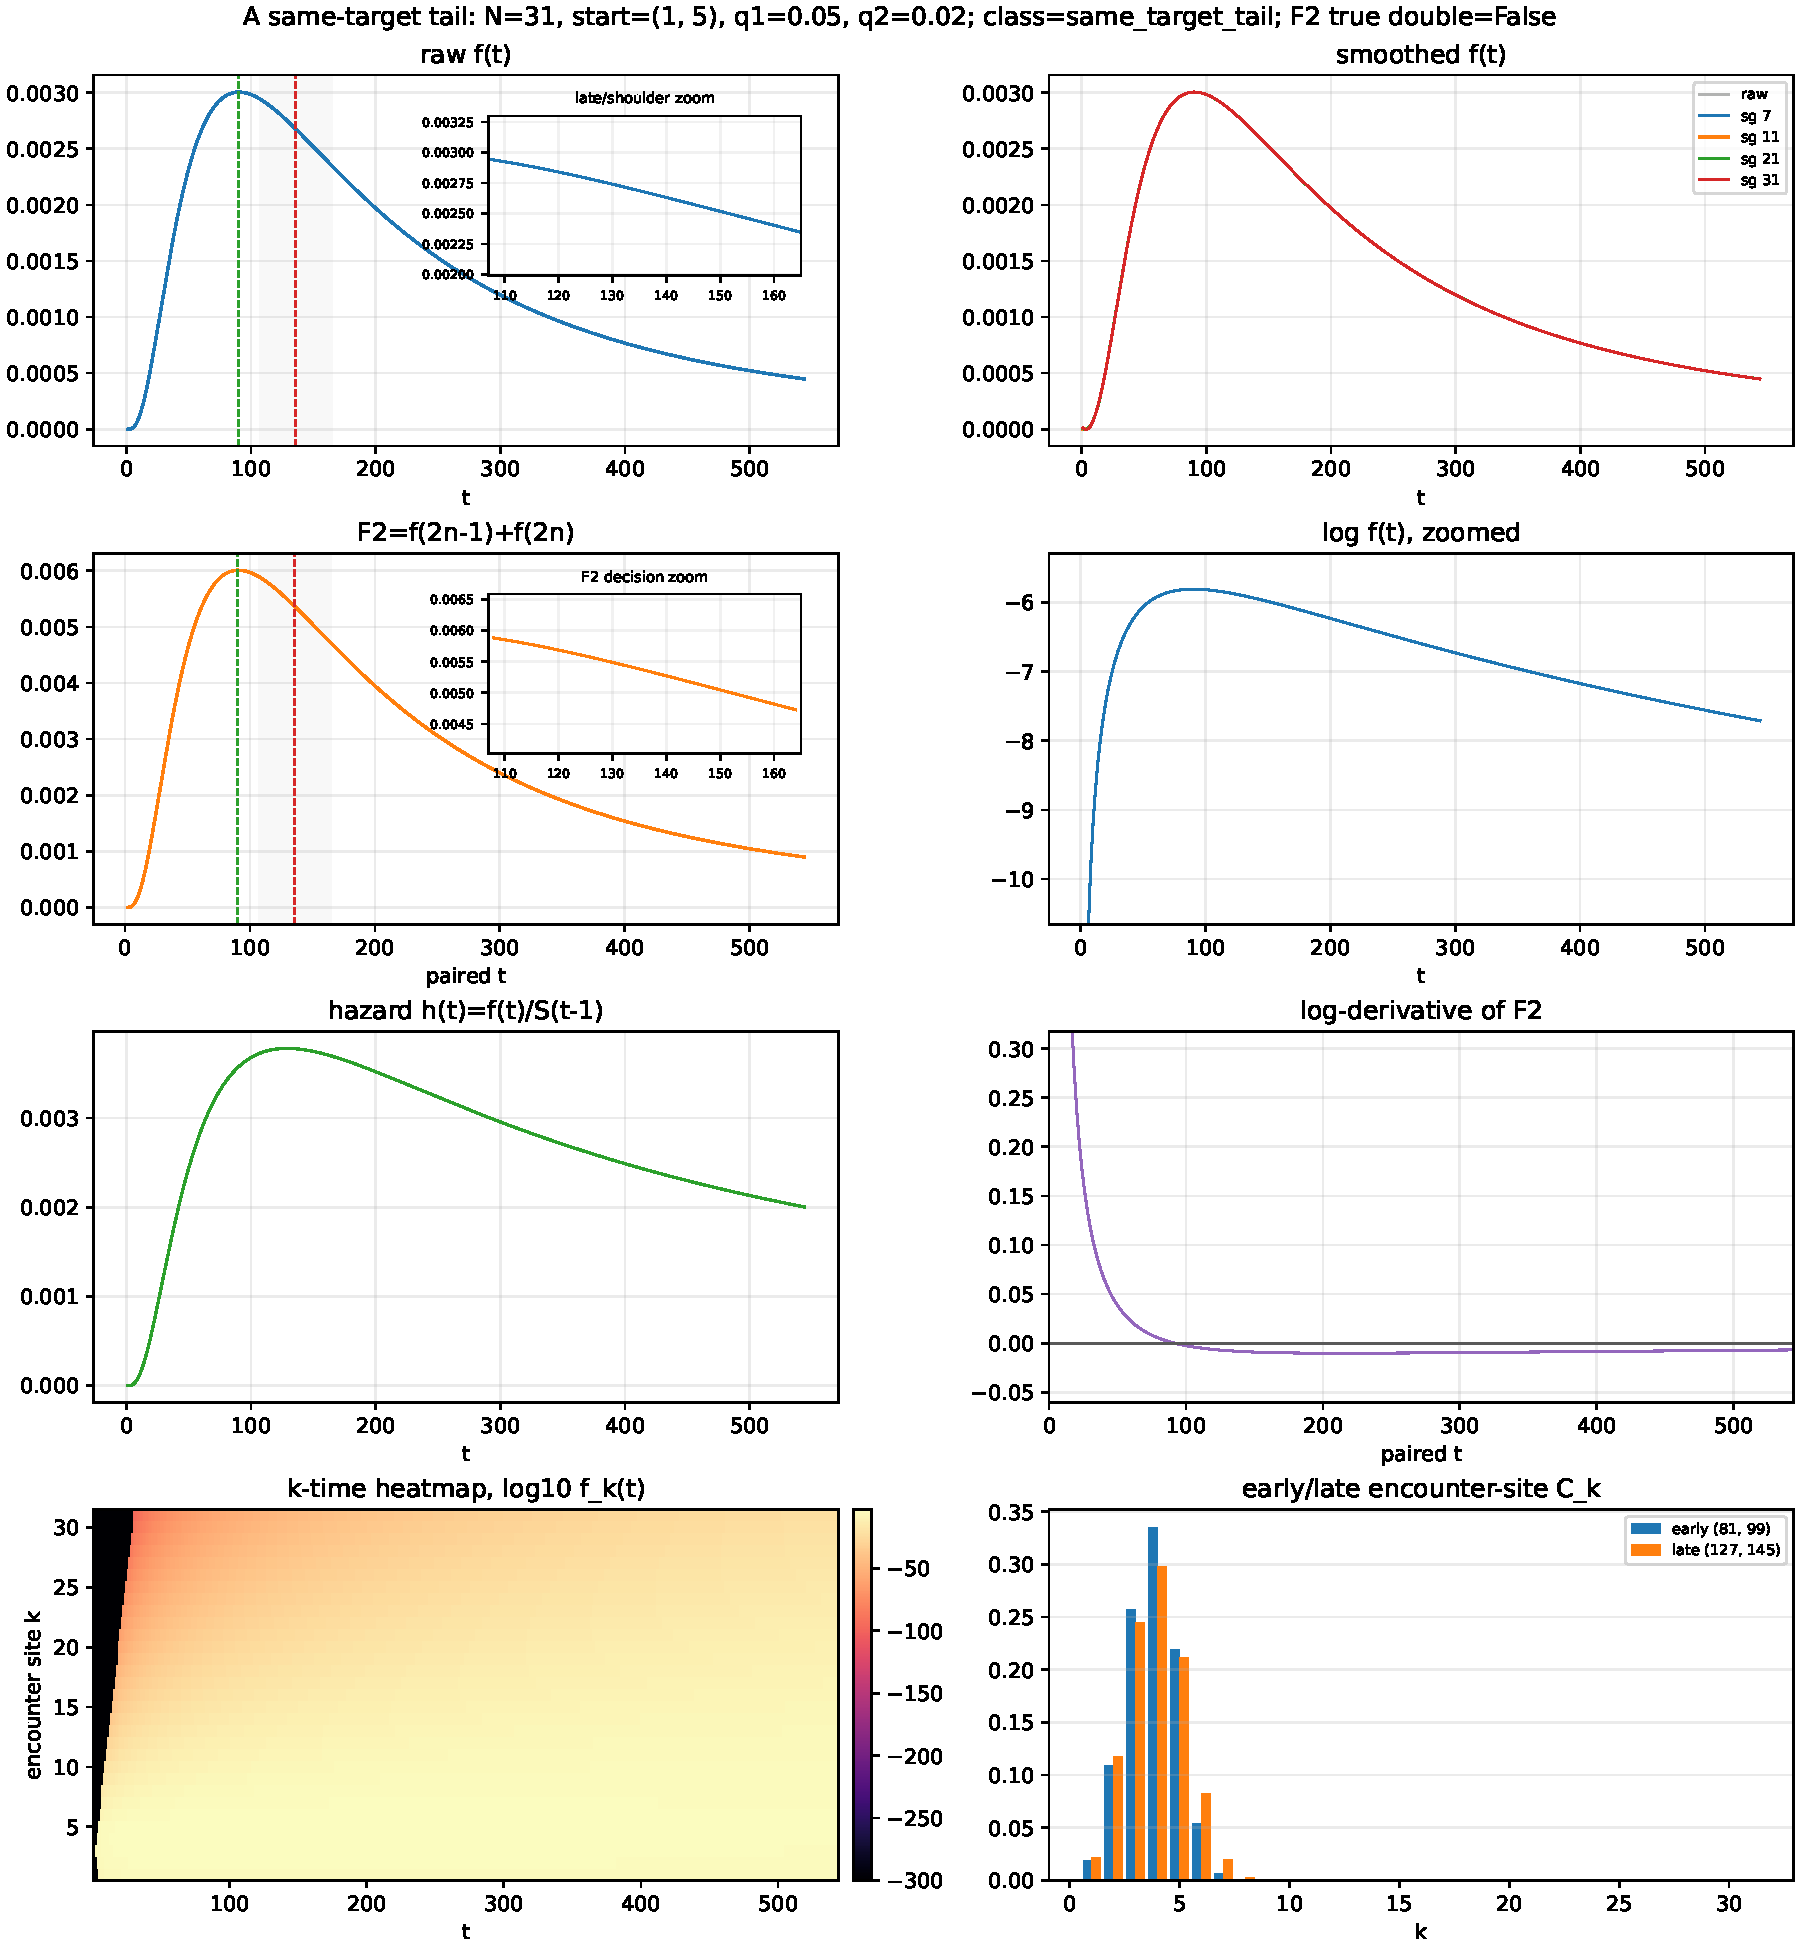
\includegraphics[width=0.96\linewidth]{A_boundary_1_5.pdf}
  \caption{Full diagnostics for case A.}
\end{figure}

\begin{figure}[p]
  \centering
  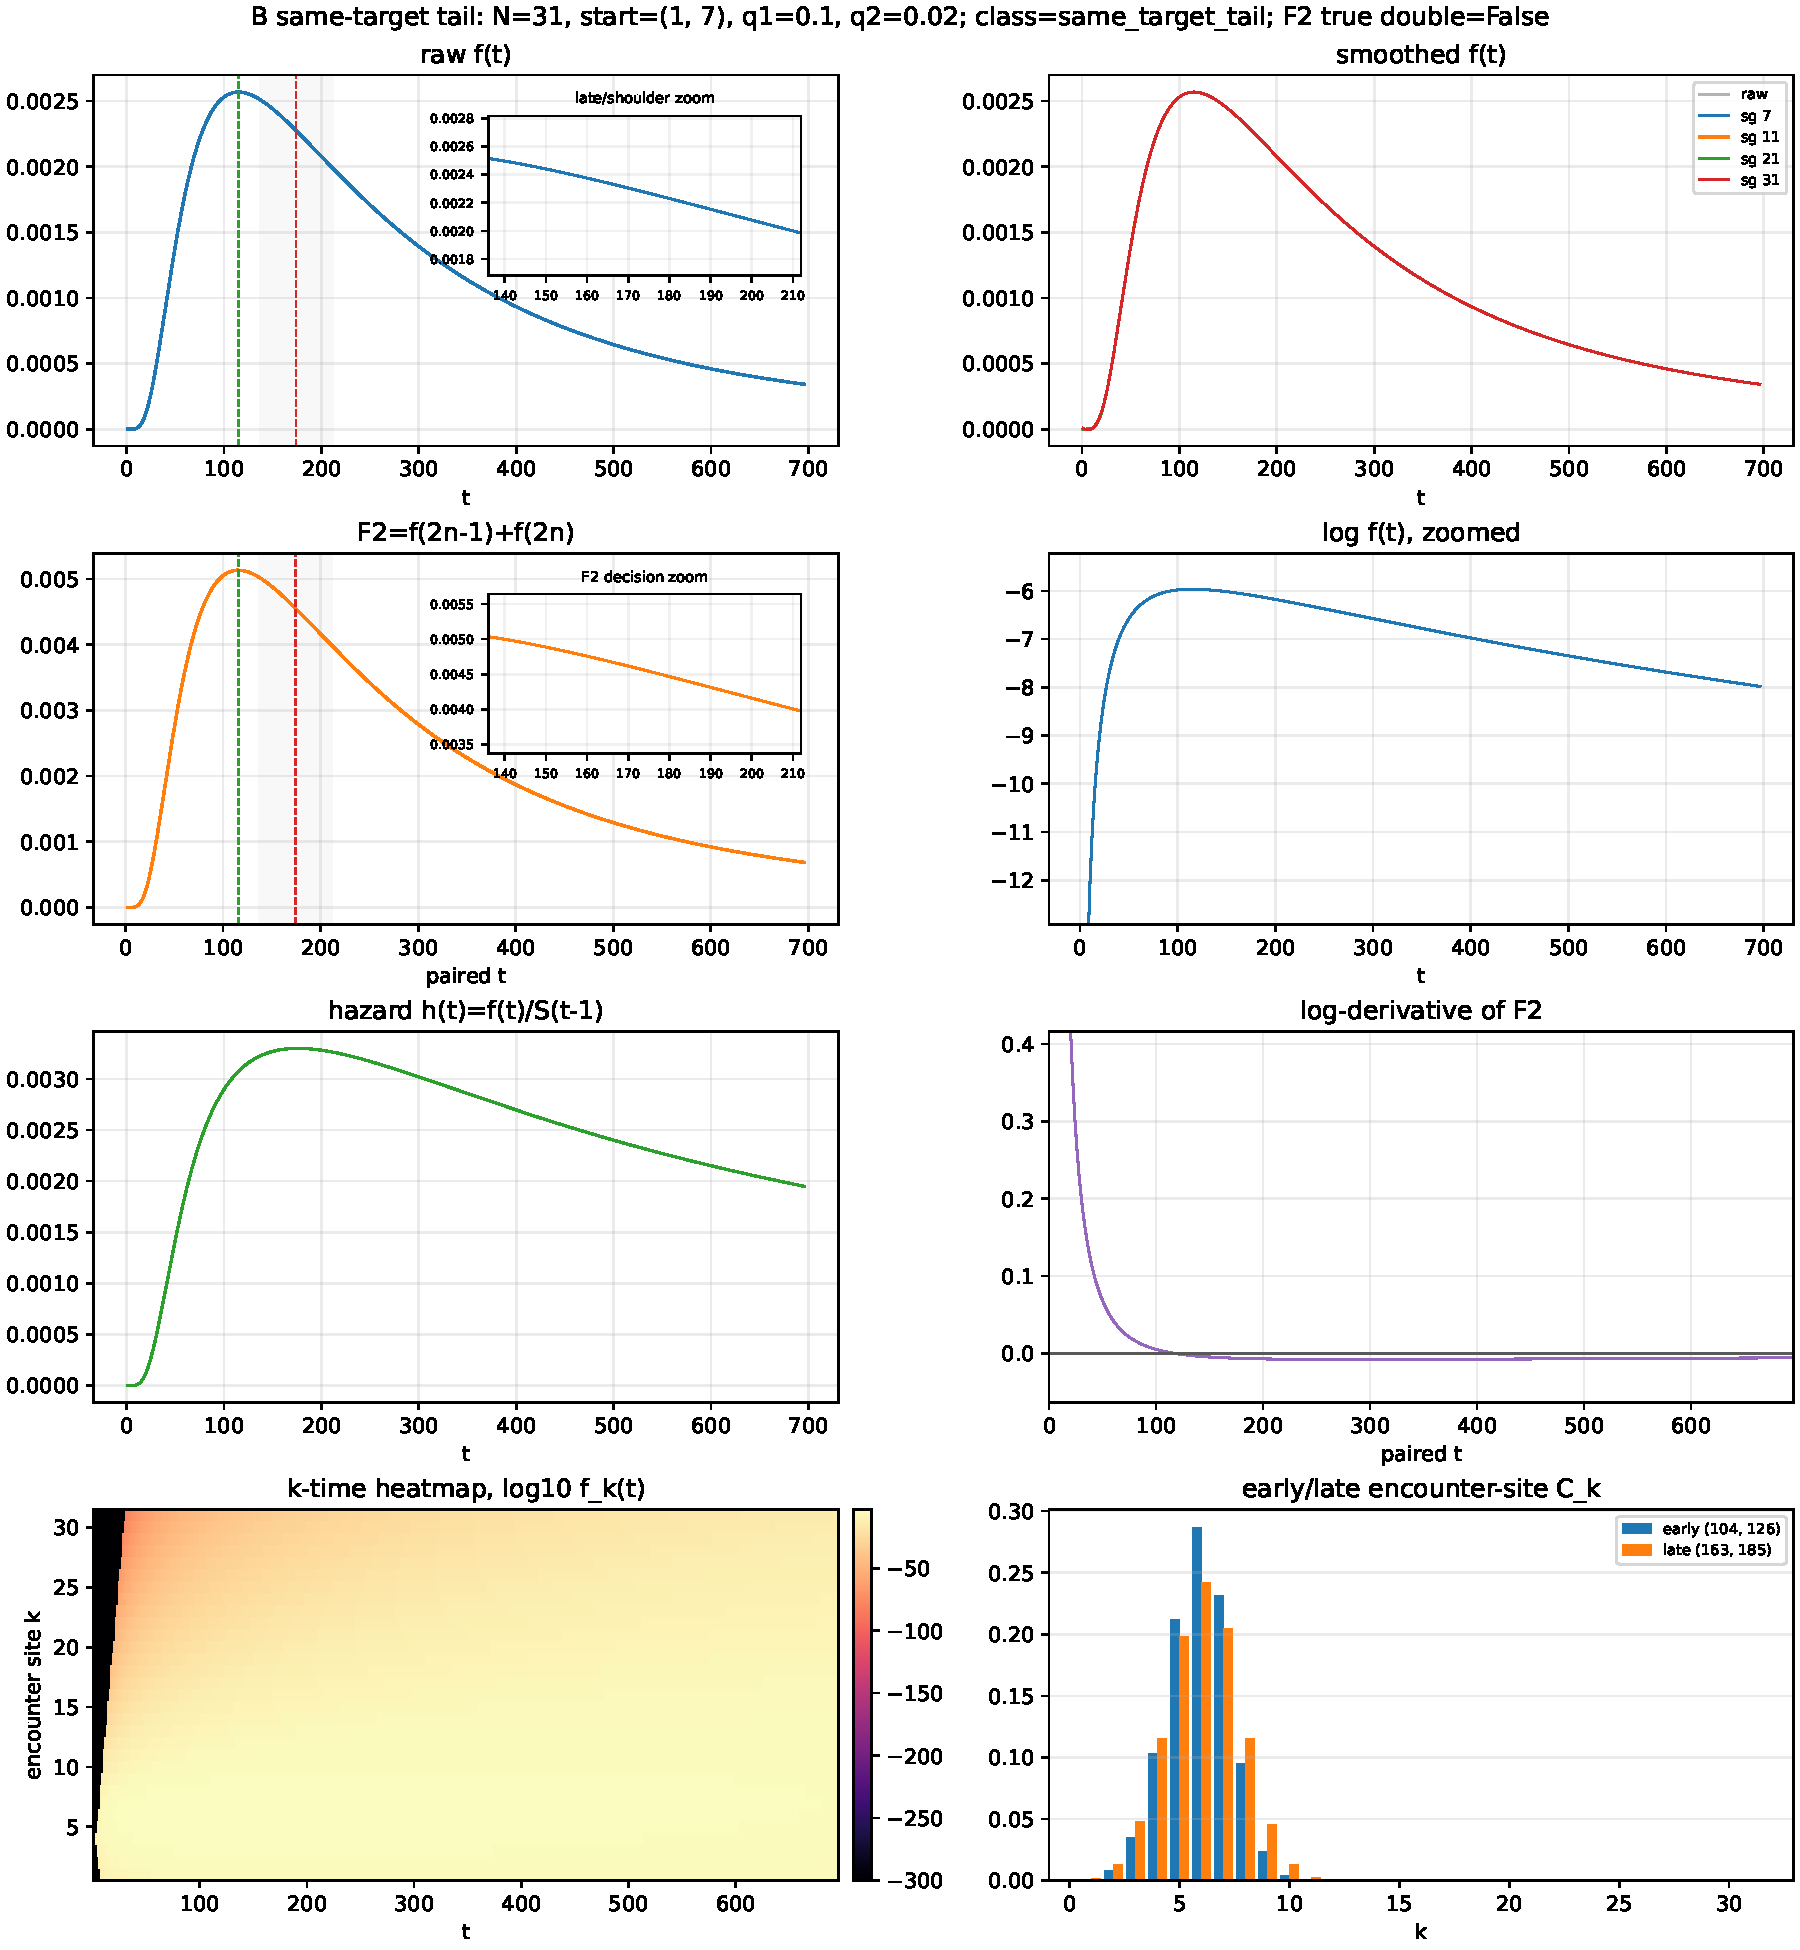
\includegraphics[width=0.96\linewidth]{B_boundary_1_7.pdf}
  \caption{Full diagnostics for case B.}
\end{figure}

\begin{figure}[p]
  \centering
  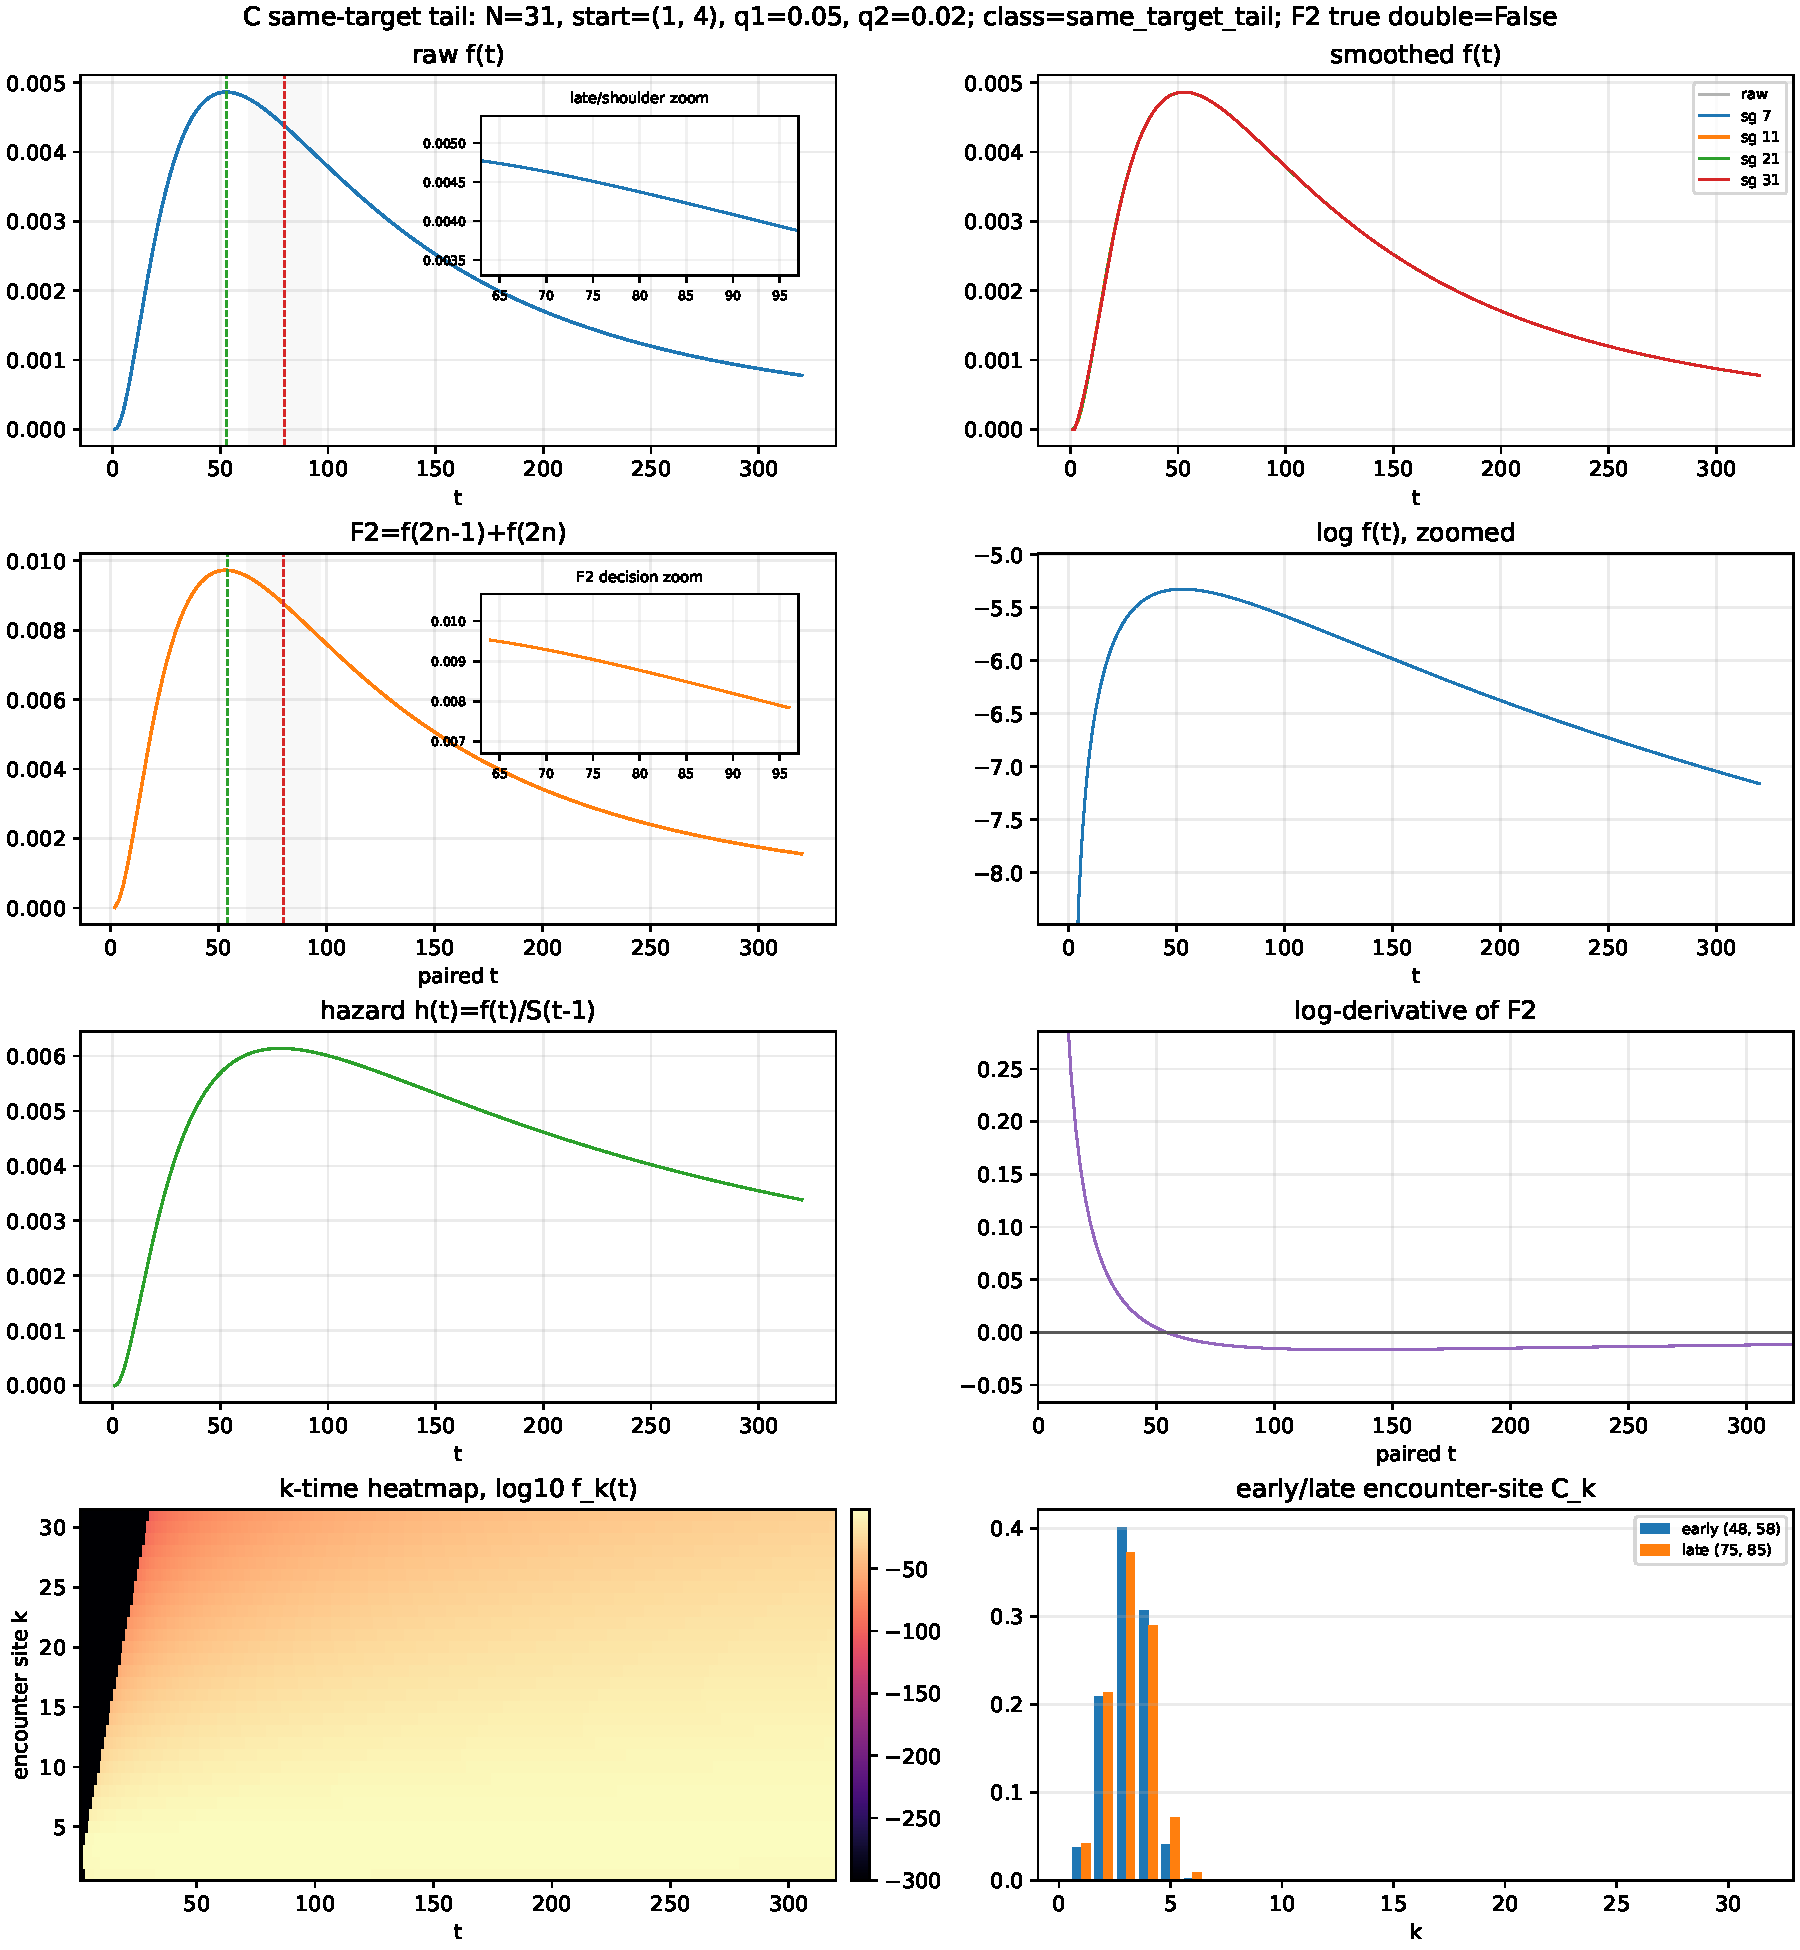
\includegraphics[width=0.96\linewidth]{C_boundary_1_4.pdf}
  \caption{Full diagnostics for case C.}
\end{figure}

\begin{figure}[p]
  \centering
  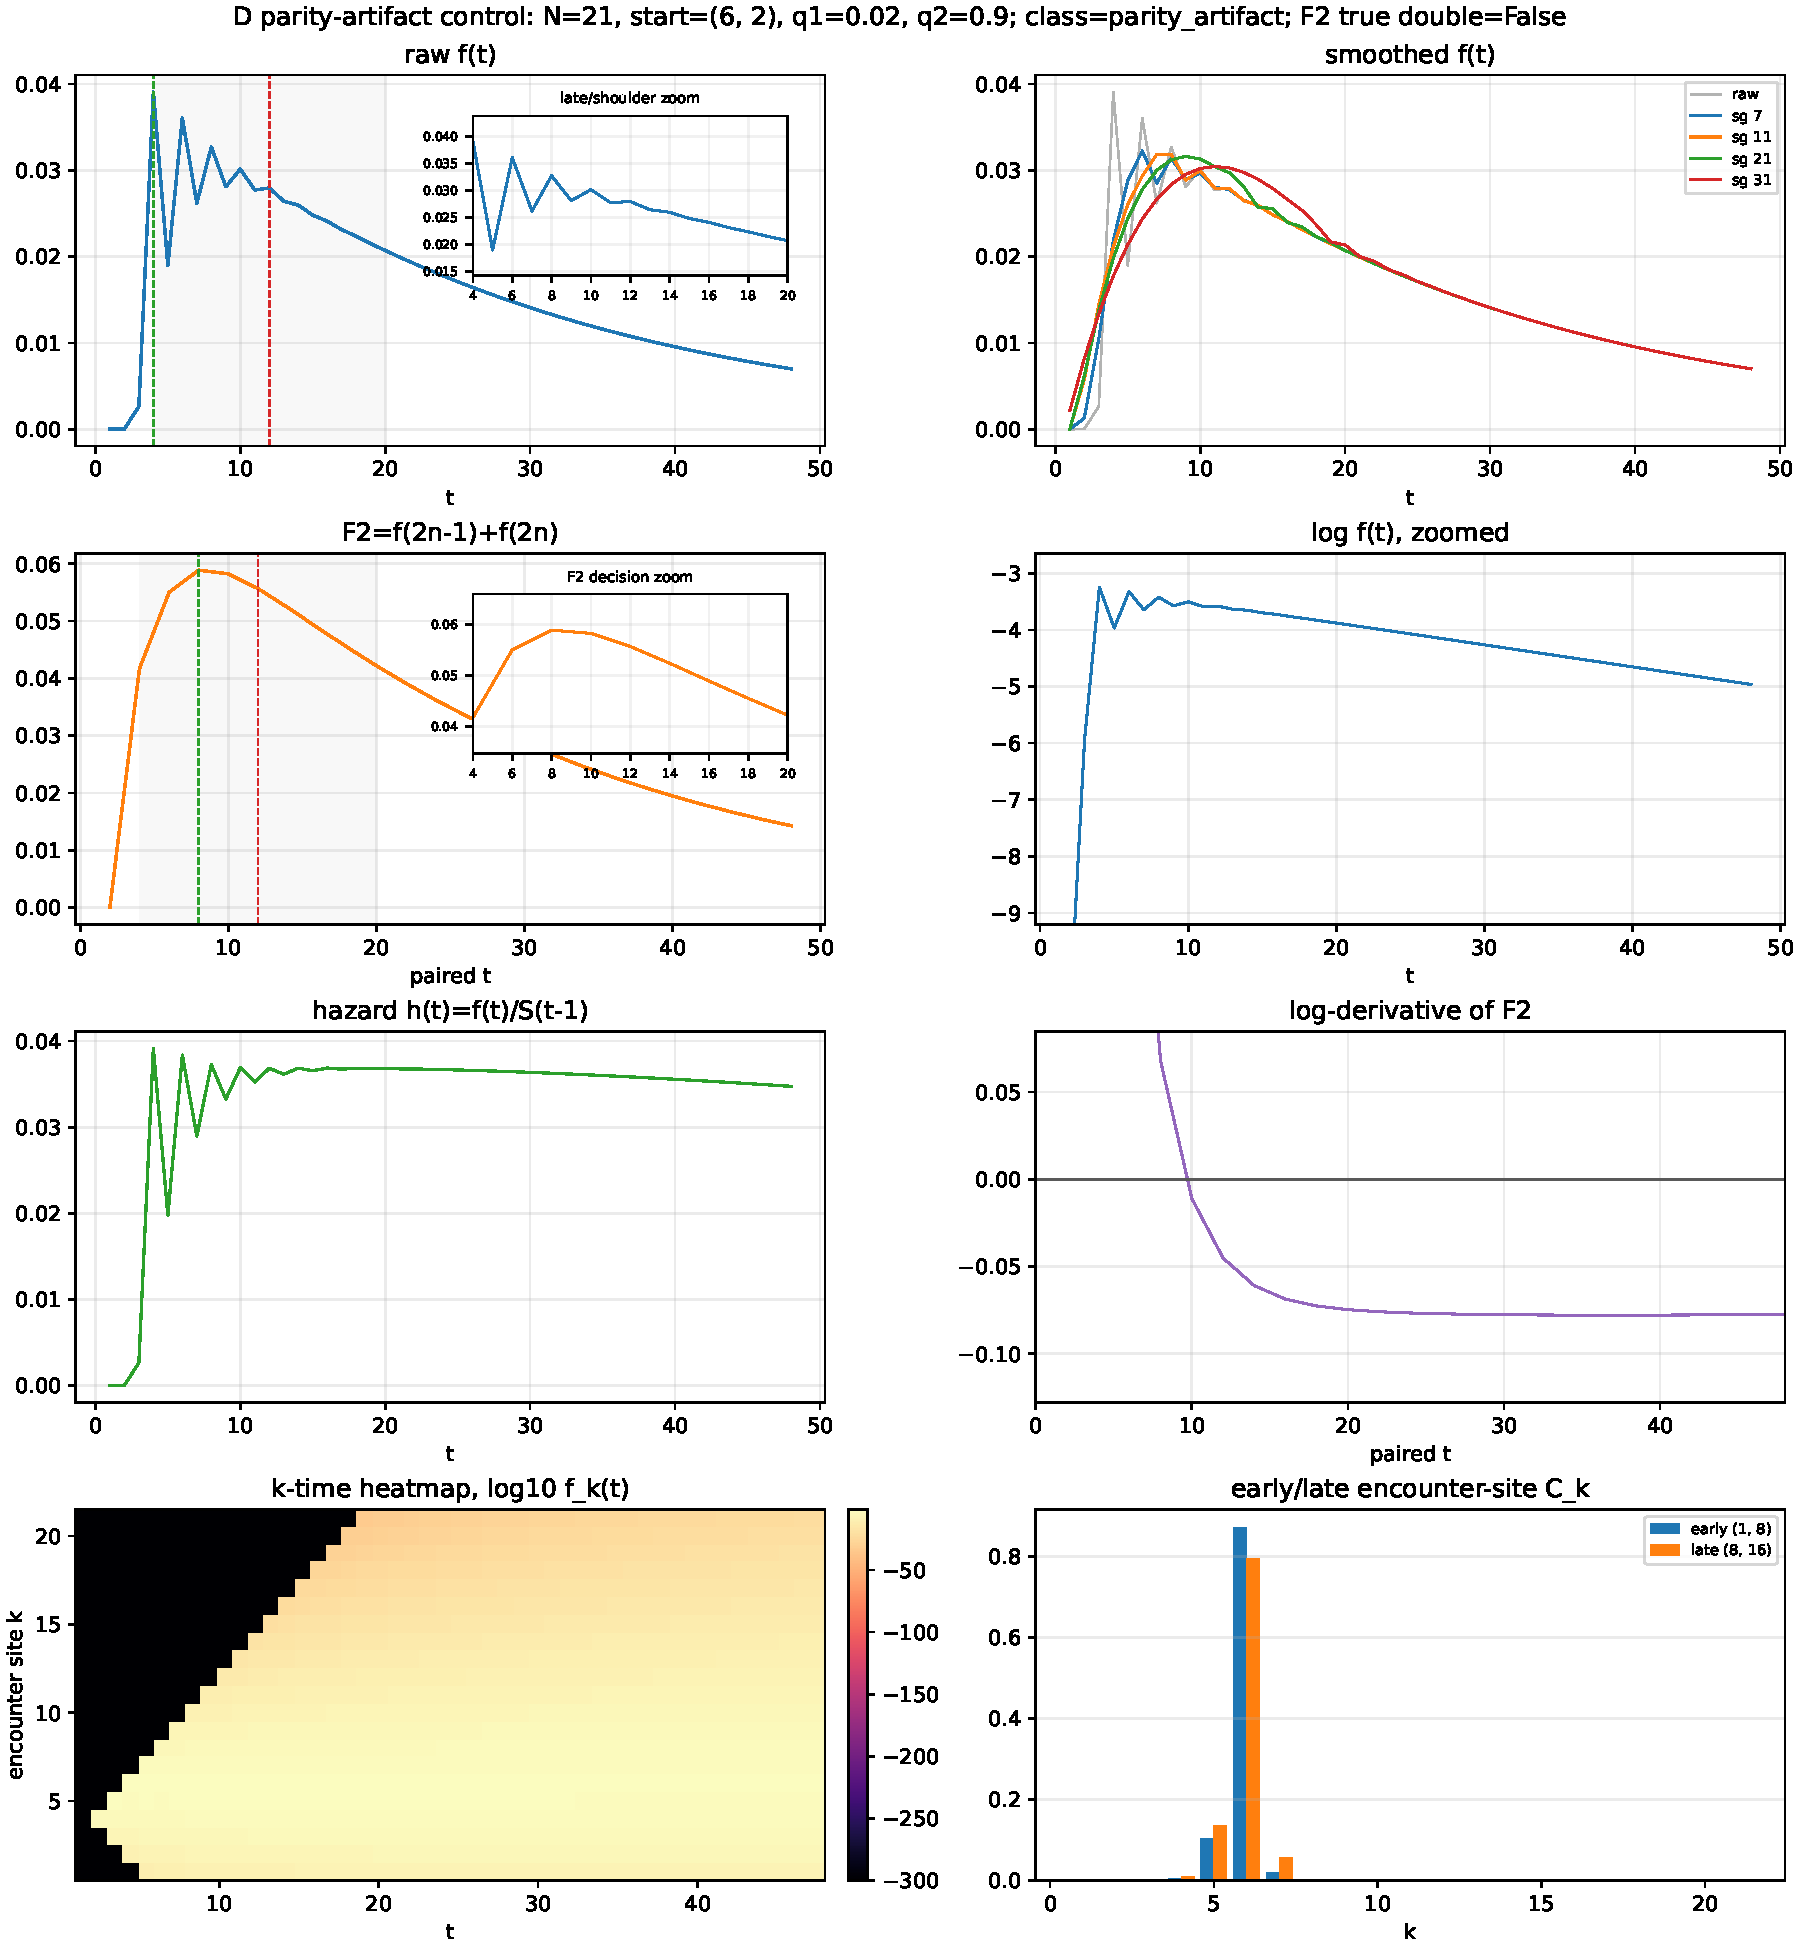
\includegraphics[width=0.96\linewidth]{D_negative_control.pdf}
  \caption{Full diagnostics for the Stage-1 negative control.}
\end{figure}

\begin{figure}[p]
  \centering
  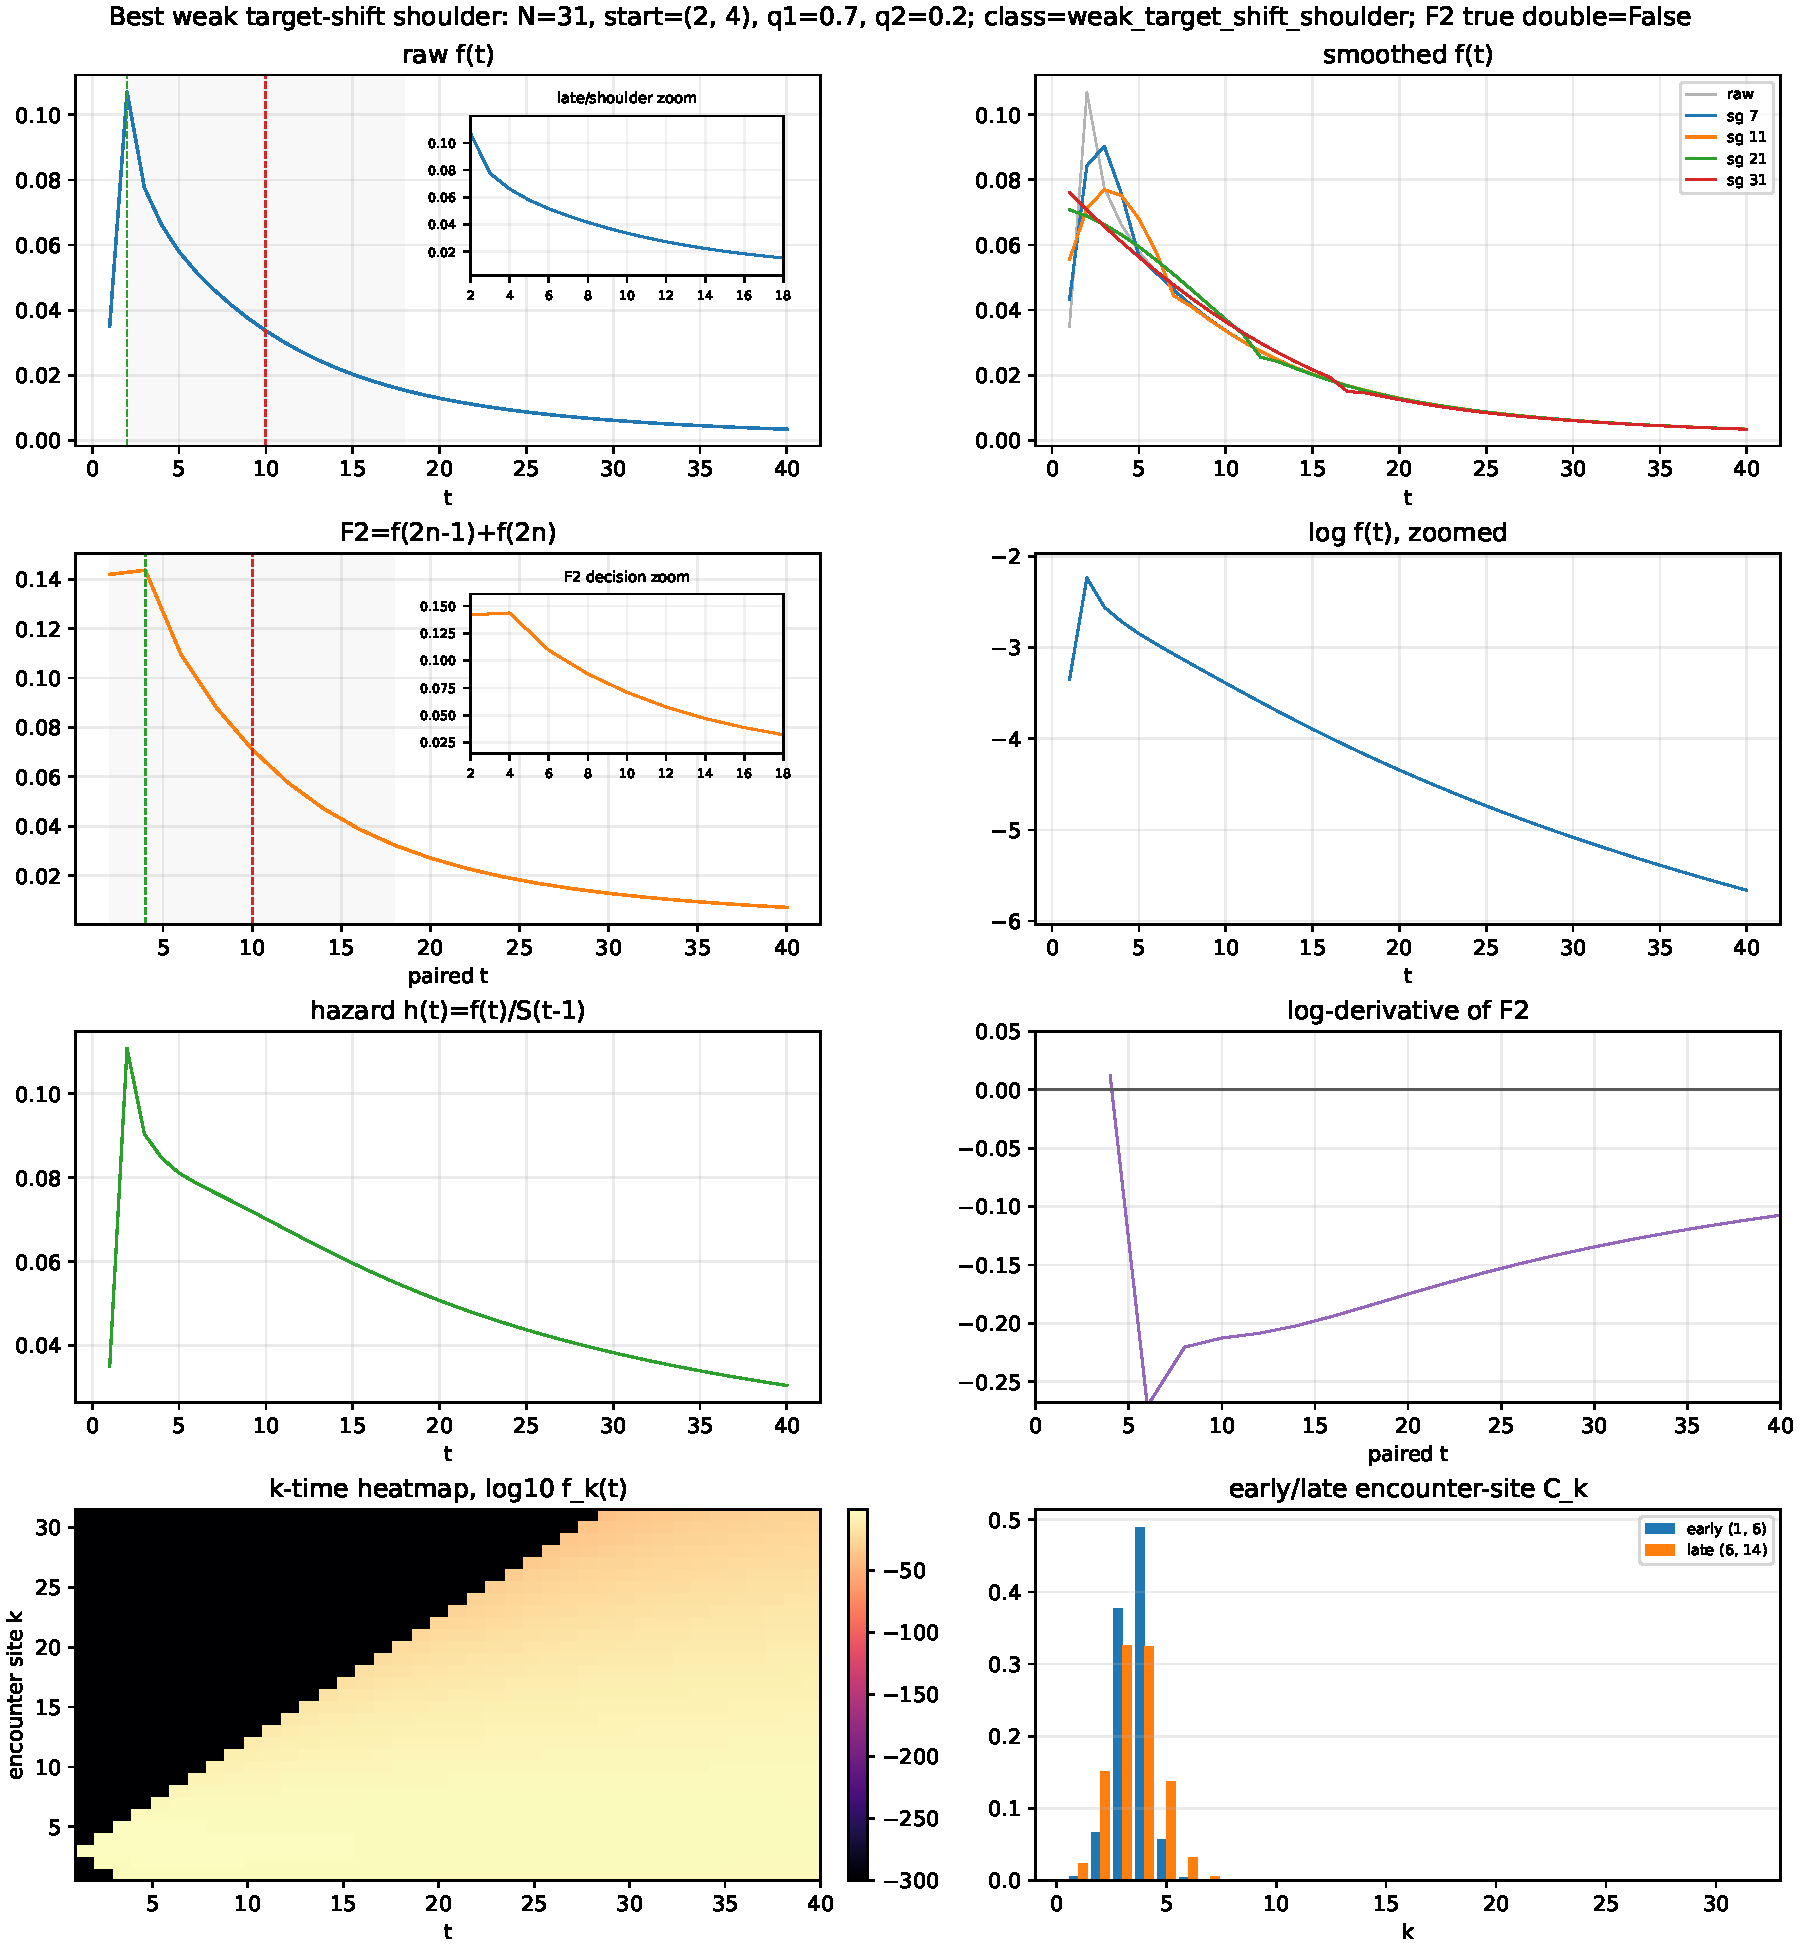
\includegraphics[width=0.96\linewidth]{E_target_shift_2_4.pdf}
  \caption{Full diagnostics for the best weak target-shift shoulder.}
\end{figure}

\section*{Reproducibility}
The final report is regenerated from the existing Stage 1, Stage 2, and Stage
2b outputs by
\begin{Verbatim}[fontsize=\footnotesize]
PYTHONPATH=research/reports/final_multitimescale_fpt_encounter/code \
  .local/encounter-py311/bin/python -m encounter_search.finalize
\end{Verbatim}
The tests used for the final package are
\begin{Verbatim}[fontsize=\footnotesize]
.local/encounter-py311/bin/python -m pytest \
  tests/test_encounter_search.py \
  tests/test_encounter_reflecting_mean_validation.py \
  tests/test_encounter_green_formula_comparison.py -q
\end{Verbatim}

\end{document}
